\section{Appendix}\label{sec:appendix}

\begin{lstlisting}[caption={VisMo Ontologie in der letzten (englischen) Version.},label={lst:vismo},captionpos=b,language=xml]
<?xml version="1.0"?>
<rdf:RDF xmlns="http://visit.de/ontologies/vismo/"
     xml:base="http://visit.de/ontologies/vismo/"
     xmlns:rdf="http://www.w3.org/1999/02/22-rdf-syntax-ns#"
     xmlns:ns="http://www.w3.org/2003/06/sw-vocab-status/ns#"
     xmlns:owl="http://www.w3.org/2002/07/owl#"
     xmlns:xml="http://www.w3.org/XML/1998/namespace"
     xmlns:xsd="http://www.w3.org/2001/XMLSchema#"
     xmlns:skos="http://www.w3.org/2004/02/skos/core#"
     xmlns:rdfs="http://www.w3.org/2000/01/rdf-schema#"
     xmlns:wot="http://xmlns.com/wot/0.1/"
     xmlns:foaf="http://xmlns.com/foaf/0.1/"
     xmlns:dc="http://purl.org/dc/elements/1.1/">
    <owl:Ontology rdf:about="http://visit.de/ontologies/vismo/">
        <owl:versionIRI rdf:resource="http://visit.de/ontologies/vismo/0.4.5/"/>
        <owl:imports rdf:resource="http://erlangen-crm.org/170309/"/>
        <owl:imports rdf:resource="http://xmlns.com/foaf/0.1/"/>
    </owl:Ontology>
    


    <!-- 
    ///////////////////////////////////////////////////////////////////////////////////////
    //
    // Object Properties
    //
    ///////////////////////////////////////////////////////////////////////////////////////
     -->

    


    <!-- http://visit.de/ontologies/vismo/containsEntry -->

    <owl:ObjectProperty rdf:about="http://visit.de/ontologies/vismo/containsEntry">
        <rdfs:subPropertyOf rdf:resource="http://www.w3.org/2002/07/owl#topObjectProperty"/>
        <owl:inverseOf rdf:resource="http://visit.de/ontologies/vismo/isEntryIn"/>
        <rdfs:domain rdf:resource="http://visit.de/ontologies/vismo/Reference"/>
        <rdfs:range rdf:resource="http://visit.de/ontologies/vismo/ReferenceEntry"/>
        <rdfs:comment>Reference from a vismo:Reference to a contained vismo:ReferenceEntry.</rdfs:comment>
        <rdfs:label>contains entry</rdfs:label>
    </owl:ObjectProperty>
    


    <!-- http://visit.de/ontologies/vismo/employsTraderoute -->

    <owl:ObjectProperty rdf:about="http://visit.de/ontologies/vismo/employsTraderoute">
        <rdfs:subPropertyOf rdf:resource="http://www.w3.org/2002/07/owl#topObjectProperty"/>
        <owl:inverseOf rdf:resource="http://visit.de/ontologies/vismo/forTrade"/>
        <rdfs:domain rdf:resource="http://visit.de/ontologies/vismo/Trade"/>
        <rdfs:range rdf:resource="http://visit.de/ontologies/vismo/Traderoute"/>
        <rdfs:comment>Refers from a vismo:Trade to the vismo:TradeRoute that the trade is fullfilled on.</rdfs:comment>
        <rdfs:label>employs traderoute</rdfs:label>
    </owl:ObjectProperty>
    


    <!-- http://visit.de/ontologies/vismo/endLocation -->

    <owl:ObjectProperty rdf:about="http://visit.de/ontologies/vismo/endLocation">
        <rdfs:subPropertyOf rdf:resource="http://visit.de/ontologies/vismo/routeLocation"/>
        <rdfs:comment>Refers from a traderoute to the vismo:City that represents the ending point for the route.</rdfs:comment>
        <rdfs:label>end location</rdfs:label>
    </owl:ObjectProperty>
    


    <!-- http://visit.de/ontologies/vismo/entryIsAbout -->

    <owl:ObjectProperty rdf:about="http://visit.de/ontologies/vismo/entryIsAbout">
        <rdfs:subPropertyOf rdf:resource="http://www.w3.org/2002/07/owl#topObjectProperty"/>
        <owl:inverseOf rdf:resource="http://visit.de/ontologies/vismo/referencedByEntry"/>
        <rdfs:domain rdf:resource="http://visit.de/ontologies/vismo/ReferenceEntry"/>
        <rdfs:range rdf:resource="http://visit.de/ontologies/vismo/Resource"/>
        <rdfs:comment>Reference from a vismo:ReferenceEntry to a vismo:Resource, associating the describing nature of the associated vismo:Reference.</rdfs:comment>
        <rdfs:label>entry is about</rdfs:label>
    </owl:ObjectProperty>
    


    <!-- http://visit.de/ontologies/vismo/forTrade -->

    <owl:ObjectProperty rdf:about="http://visit.de/ontologies/vismo/forTrade">
        <rdfs:subPropertyOf rdf:resource="http://www.w3.org/2002/07/owl#topObjectProperty"/>
        <rdfs:domain rdf:resource="http://visit.de/ontologies/vismo/Traderoute"/>
        <rdfs:range rdf:resource="http://visit.de/ontologies/vismo/Trade"/>
        <rdfs:comment>Refers from a vismo:TradeRoute to the vismo:Trade resource that illustrates the trading on the given route.</rdfs:comment>
        <rdfs:label>for trade</rdfs:label>
    </owl:ObjectProperty>
    


    <!-- http://visit.de/ontologies/vismo/hasDigitalRepresentation -->

    <owl:ObjectProperty rdf:about="http://visit.de/ontologies/vismo/hasDigitalRepresentation">
        <rdfs:subPropertyOf rdf:resource="http://www.w3.org/2002/07/owl#topObjectProperty"/>
        <owl:inverseOf rdf:resource="http://visit.de/ontologies/vismo/representsDigitally"/>
        <rdfs:domain rdf:resource="http://visit.de/ontologies/vismo/Resource"/>
        <rdfs:range rdf:resource="http://visit.de/ontologies/vismo/DigitalRepresentation"/>
        <rdfs:comment>Links from a vismo:Resource (so an object that can be further specified in the ViSIT context) to a digital representation of it, e.g. a picture that shows the respective resource, a 3D model, etc.</rdfs:comment>
        <rdfs:label>has digital representation</rdfs:label>
    </owl:ObjectProperty>
    


    <!-- http://visit.de/ontologies/vismo/interactionSource -->

    <owl:ObjectProperty rdf:about="http://visit.de/ontologies/vismo/interactionSource">
        <rdfs:subPropertyOf rdf:resource="http://www.w3.org/2002/07/owl#topObjectProperty"/>
        <rdfs:domain rdf:resource="http://visit.de/ontologies/vismo/MiscellaneousInteraction"/>
        <rdfs:range rdf:resource="http://visit.de/ontologies/vismo/Resource"/>
        <rdfs:label>interaction source</rdfs:label>
    </owl:ObjectProperty>
    


    <!-- http://visit.de/ontologies/vismo/interactionTarget -->

    <owl:ObjectProperty rdf:about="http://visit.de/ontologies/vismo/interactionTarget">
        <rdfs:subPropertyOf rdf:resource="http://www.w3.org/2002/07/owl#topObjectProperty"/>
        <rdfs:domain rdf:resource="http://visit.de/ontologies/vismo/Resource"/>
        <rdfs:range rdf:resource="http://visit.de/ontologies/vismo/MiscellaneousInteraction"/>
        <rdfs:label>interaction target</rdfs:label>
    </owl:ObjectProperty>
    


    <!-- http://visit.de/ontologies/vismo/interstation -->

    <owl:ObjectProperty rdf:about="http://visit.de/ontologies/vismo/interstation">
        <rdfs:subPropertyOf rdf:resource="http://visit.de/ontologies/vismo/routeLocation"/>
        <rdfs:comment>Refers from a traderoute to the vismo:City that represents a interstation for the route.</rdfs:comment>
        <rdfs:label>interstation</rdfs:label>
    </owl:ObjectProperty>
    


    <!-- http://visit.de/ontologies/vismo/isEntryIn -->

    <owl:ObjectProperty rdf:about="http://visit.de/ontologies/vismo/isEntryIn">
        <rdfs:subPropertyOf rdf:resource="http://www.w3.org/2002/07/owl#topObjectProperty"/>
        <rdfs:domain rdf:resource="http://visit.de/ontologies/vismo/ReferenceEntry"/>
        <rdfs:range rdf:resource="http://visit.de/ontologies/vismo/Reference"/>
        <rdfs:comment>Reference from a vismo:ReferenceEntry to its encompassing vismo:Resource.</rdfs:comment>
        <rdfs:label>is entry in</rdfs:label>
    </owl:ObjectProperty>
    


    <!-- http://visit.de/ontologies/vismo/partOfTradeRoute -->

    <owl:ObjectProperty rdf:about="http://visit.de/ontologies/vismo/partOfTradeRoute">
        <rdfs:subPropertyOf rdf:resource="http://www.w3.org/2002/07/owl#topObjectProperty"/>
        <owl:inverseOf rdf:resource="http://visit.de/ontologies/vismo/routeLocation"/>
        <rdfs:domain rdf:resource="http://visit.de/ontologies/vismo/Place"/>
        <rdfs:range rdf:resource="http://visit.de/ontologies/vismo/Traderoute"/>
        <rdfs:comment>Refers from a vismo:City to a/multiple vismo:TradeRoute resource, indicating the given city is part of a trade route and therefore its associated trade.</rdfs:comment>
        <rdfs:label>part of trade route</rdfs:label>
    </owl:ObjectProperty>
    


    <!-- http://visit.de/ontologies/vismo/reference -->

    <owl:ObjectProperty rdf:about="http://visit.de/ontologies/vismo/reference">
        <rdfs:subPropertyOf rdf:resource="http://www.w3.org/2002/07/owl#topObjectProperty"/>
        <owl:inverseOf rdf:resource="http://visit.de/ontologies/vismo/referencedBy"/>
        <rdfs:domain rdf:resource="http://visit.de/ontologies/vismo/Resource"/>
        <rdfs:range rdf:resource="http://visit.de/ontologies/vismo/Reference"/>
        <rdfs:comment>Issues that the referenced vismo:Reference contains further and descriptive information about the given vismo:Resource entity.</rdfs:comment>
        <rdfs:label>reference</rdfs:label>
    </owl:ObjectProperty>
    


    <!-- http://visit.de/ontologies/vismo/referencedBy -->

    <owl:ObjectProperty rdf:about="http://visit.de/ontologies/vismo/referencedBy">
        <rdfs:subPropertyOf rdf:resource="http://www.w3.org/2002/07/owl#topObjectProperty"/>
        <rdfs:domain rdf:resource="http://visit.de/ontologies/vismo/Reference"/>
        <rdfs:range rdf:resource="http://visit.de/ontologies/vismo/Resource"/>
        <rdfs:comment>Refers to the vismo:Resource entities that reference this vismo:Reference and therefore this entity contains further and descriptive information about the resource entities.</rdfs:comment>
        <rdfs:label>referenced by</rdfs:label>
    </owl:ObjectProperty>
    


    <!-- http://visit.de/ontologies/vismo/referencedByEntry -->

    <owl:ObjectProperty rdf:about="http://visit.de/ontologies/vismo/referencedByEntry">
        <rdfs:subPropertyOf rdf:resource="http://www.w3.org/2002/07/owl#topObjectProperty"/>
        <rdfs:domain rdf:resource="http://visit.de/ontologies/vismo/Resource"/>
        <rdfs:range rdf:resource="http://visit.de/ontologies/vismo/ReferenceEntry"/>
        <rdfs:comment>Reference from a vismo:Resource to a given vismo:ReferenceEntry, indicating that the associated vismo:Reference contains information about the former.</rdfs:comment>
        <rdfs:label>referenced by entry</rdfs:label>
    </owl:ObjectProperty>
    


    <!-- http://visit.de/ontologies/vismo/representsDigitally -->

    <owl:ObjectProperty rdf:about="http://visit.de/ontologies/vismo/representsDigitally">
        <rdfs:subPropertyOf rdf:resource="http://www.w3.org/2002/07/owl#topObjectProperty"/>
        <rdfs:domain rdf:resource="http://visit.de/ontologies/vismo/DigitalRepresentation"/>
        <rdfs:range rdf:resource="http://visit.de/ontologies/vismo/Resource"/>
        <rdfs:comment>Refers from a given digital representation (a picture, 3D model, etc.) back to the vismo:Resource that it originally represents.</rdfs:comment>
        <rdfs:label>represents digitally</rdfs:label>
    </owl:ObjectProperty>
    


    <!-- http://visit.de/ontologies/vismo/routeLocation -->

    <owl:ObjectProperty rdf:about="http://visit.de/ontologies/vismo/routeLocation">
        <rdfs:subPropertyOf rdf:resource="http://www.w3.org/2002/07/owl#topObjectProperty"/>
        <rdfs:domain rdf:resource="http://visit.de/ontologies/vismo/Traderoute"/>
        <rdfs:range rdf:resource="http://visit.de/ontologies/vismo/Place"/>
        <rdfs:comment>Refers (with different sub-properties) from a vismo:TradeRoute to a vismo:City that is located on said route.</rdfs:comment>
        <rdfs:label>route location</rdfs:label>
    </owl:ObjectProperty>
    


    <!-- http://visit.de/ontologies/vismo/startLocation -->

    <owl:ObjectProperty rdf:about="http://visit.de/ontologies/vismo/startLocation">
        <rdfs:subPropertyOf rdf:resource="http://visit.de/ontologies/vismo/routeLocation"/>
        <rdfs:comment>Refers from a traderoute to the vismo:City that represents the starting point for the route.</rdfs:comment>
        <rdfs:label>start location</rdfs:label>
    </owl:ObjectProperty>
    


    <!-- 
    ///////////////////////////////////////////////////////////////////////////////////////
    //
    // Data properties
    //
    ///////////////////////////////////////////////////////////////////////////////////////
     -->

    


    <!-- http://visit.de/ontologies/vismo/buildingHistory -->

    <owl:DatatypeProperty rdf:about="http://visit.de/ontologies/vismo/buildingHistory">
        <rdfs:subPropertyOf rdf:resource="http://www.w3.org/2002/07/owl#topDataProperty"/>
        <rdfs:domain rdf:resource="http://visit.de/ontologies/vismo/Architecture"/>
        <rdfs:range rdf:resource="http://www.w3.org/2000/01/rdf-schema#Literal"/>
        <rdfs:comment>Property used to (freely) describe the building history of a vismo:Architecture entity.</rdfs:comment>
        <rdfs:label>building history</rdfs:label>
    </owl:DatatypeProperty>
    


    <!-- http://visit.de/ontologies/vismo/comment -->

    <owl:DatatypeProperty rdf:about="http://visit.de/ontologies/vismo/comment">
        <rdfs:subPropertyOf rdf:resource="http://www.w3.org/2002/07/owl#topDataProperty"/>
        <rdfs:domain rdf:resource="http://visit.de/ontologies/vismo/Resource"/>
        <rdfs:range rdf:resource="http://www.w3.org/2000/01/rdf-schema#Literal"/>
        <rdfs:comment rdf:datatype="http://www.w3.org/2001/XMLSchema#string">This is a comment about a given vismo entity.</rdfs:comment>
        <rdfs:isDefinedBy rdf:datatype="http://www.w3.org/2001/XMLSchema#string">http://visit.de/ontologies/vismo</rdfs:isDefinedBy>
        <rdfs:label rdf:datatype="http://www.w3.org/2001/XMLSchema#string">comment</rdfs:label>
    </owl:DatatypeProperty>
    


    <!-- http://visit.de/ontologies/vismo/description -->

    <owl:DatatypeProperty rdf:about="http://visit.de/ontologies/vismo/description">
        <rdfs:subPropertyOf rdf:resource="http://www.w3.org/2002/07/owl#topDataProperty"/>
        <rdfs:domain rdf:resource="http://visit.de/ontologies/vismo/Resource"/>
        <rdfs:range rdf:resource="http://www.w3.org/2000/01/rdf-schema#Literal"/>
        <rdfs:comment rdf:datatype="http://www.w3.org/2001/XMLSchema#string">This property defines a (historical) description for a vismo entity.</rdfs:comment>
        <rdfs:isDefinedBy rdf:datatype="http://www.w3.org/2001/XMLSchema#string">http://visit.de/ontologies/vismo/</rdfs:isDefinedBy>
        <rdfs:label rdf:datatype="http://www.w3.org/2001/XMLSchema#string">description</rdfs:label>
    </owl:DatatypeProperty>
    


    <!-- http://visit.de/ontologies/vismo/entryPages -->

    <owl:DatatypeProperty rdf:about="http://visit.de/ontologies/vismo/entryPages">
        <rdfs:subPropertyOf rdf:resource="http://www.w3.org/2002/07/owl#topDataProperty"/>
        <rdfs:domain rdf:resource="http://visit.de/ontologies/vismo/ReferenceEntry"/>
        <rdfs:range rdf:resource="http://www.w3.org/2000/01/rdf-schema#Literal"/>
        <rdfs:comment>The range of pages that a given vismo:ReferenceEntry references of a vismo:Reference entity.</rdfs:comment>
        <rdfs:label>entry pages</rdfs:label>
    </owl:DatatypeProperty>
    


    <!-- http://visit.de/ontologies/vismo/helpfulLinks -->

    <owl:DatatypeProperty rdf:about="http://visit.de/ontologies/vismo/helpfulLinks">
        <rdfs:subPropertyOf rdf:resource="http://www.w3.org/2002/07/owl#topDataProperty"/>
        <rdfs:domain rdf:resource="http://visit.de/ontologies/vismo/Resource"/>
        <rdfs:range rdf:resource="http://www.w3.org/2000/01/rdf-schema#Literal"/>
        <rdfs:comment>This property is used to conveniently collect links to online resources that contain further information of the associated vismo:Resource.</rdfs:comment>
        <rdfs:label>helpful links</rdfs:label>
    </owl:DatatypeProperty>
    


    <!-- http://visit.de/ontologies/vismo/iconography -->

    <owl:DatatypeProperty rdf:about="http://visit.de/ontologies/vismo/iconography">
        <rdfs:subPropertyOf rdf:resource="http://www.w3.org/2002/07/owl#topDataProperty"/>
        <rdfs:domain rdf:resource="http://visit.de/ontologies/vismo/Resource"/>
        <rdfs:range rdf:resource="http://www.w3.org/2000/01/rdf-schema#Literal"/>
        <rdfs:comment>A property to associate iconography to a given vismo:Resource entity.</rdfs:comment>
        <rdfs:label>iconography</rdfs:label>
    </owl:DatatypeProperty>
    


    <!-- http://visit.de/ontologies/vismo/innerDescription -->

    <owl:DatatypeProperty rdf:about="http://visit.de/ontologies/vismo/innerDescription">
        <rdfs:subPropertyOf rdf:resource="http://www.w3.org/2002/07/owl#topDataProperty"/>
        <rdfs:domain rdf:resource="http://visit.de/ontologies/vismo/Architecture"/>
        <rdfs:range rdf:resource="http://www.w3.org/2000/01/rdf-schema#Literal"/>
        <rdfs:comment>Property used to describe the interior of a vismo:Architecture entity.</rdfs:comment>
        <rdfs:label>inner description</rdfs:label>
    </owl:DatatypeProperty>
    


    <!-- http://visit.de/ontologies/vismo/keyword -->

    <owl:DatatypeProperty rdf:about="http://visit.de/ontologies/vismo/keyword">
        <rdfs:subPropertyOf rdf:resource="http://www.w3.org/2002/07/owl#topDataProperty"/>
        <rdfs:domain rdf:resource="http://visit.de/ontologies/vismo/Resource"/>
        <rdfs:range rdf:resource="http://www.w3.org/2000/01/rdf-schema#Literal"/>
        <rdfs:comment>This property is used to address keywords for a vismo:Resource entity. These refer to more general topics that can be addressed to anything out of the VisMo domain, for example &quot;Trade&quot;, &quot;War&quot;/&quot;Peace&quot;, or overall temporal associations.</rdfs:comment>
        <rdfs:label>keyword</rdfs:label>
    </owl:DatatypeProperty>
    


    <!-- http://visit.de/ontologies/vismo/literature -->

    <owl:DatatypeProperty rdf:about="http://visit.de/ontologies/vismo/literature">
        <rdfs:subPropertyOf rdf:resource="http://www.w3.org/2002/07/owl#topDataProperty"/>
        <rdfs:domain rdf:resource="http://visit.de/ontologies/vismo/Resource"/>
        <rdfs:range rdf:resource="http://www.w3.org/2000/01/rdf-schema#Literal"/>
        <rdfs:comment rdf:datatype="http://www.w3.org/2001/XMLSchema#string">This property defines a literature entry that contains further information about the given vismo entity.</rdfs:comment>
        <rdfs:isDefinedBy rdf:datatype="http://www.w3.org/2001/XMLSchema#string">http://visit.de/ontologies/vismo/</rdfs:isDefinedBy>
        <rdfs:label rdf:datatype="http://www.w3.org/2001/XMLSchema#string">literature</rdfs:label>
    </owl:DatatypeProperty>
    


    <!-- http://visit.de/ontologies/vismo/outerDescription -->

    <owl:DatatypeProperty rdf:about="http://visit.de/ontologies/vismo/outerDescription">
        <rdfs:subPropertyOf rdf:resource="http://www.w3.org/2002/07/owl#topDataProperty"/>
        <rdfs:domain rdf:resource="http://visit.de/ontologies/vismo/Architecture"/>
        <rdfs:range rdf:resource="http://www.w3.org/2000/01/rdf-schema#Literal"/>
        <rdfs:comment>Property used to describe the exterior of a vismo:Architecture entity.</rdfs:comment>
        <rdfs:label>outer description</rdfs:label>
    </owl:DatatypeProperty>
    


    <!-- http://visit.de/ontologies/vismo/pages -->

    <owl:DatatypeProperty rdf:about="http://visit.de/ontologies/vismo/pages">
        <rdfs:subPropertyOf rdf:resource="http://www.w3.org/2002/07/owl#topDataProperty"/>
        <rdfs:domain rdf:resource="http://visit.de/ontologies/vismo/Reference"/>
        <rdfs:range rdf:resource="http://www.w3.org/2000/01/rdf-schema#Literal"/>
        <rdfs:comment>Number of pages of a given vismo:Reference entity.</rdfs:comment>
        <rdfs:label>pages</rdfs:label>
    </owl:DatatypeProperty>
    


    <!-- http://visit.de/ontologies/vismo/publisher -->

    <owl:DatatypeProperty rdf:about="http://visit.de/ontologies/vismo/publisher">
        <rdfs:subPropertyOf rdf:resource="http://www.w3.org/2002/07/owl#topDataProperty"/>
        <rdfs:domain rdf:resource="http://visit.de/ontologies/vismo/Reference"/>
        <rdfs:range rdf:resource="http://www.w3.org/2000/01/rdf-schema#Literal"/>
        <rdfs:comment>The publisher of the given vismo:Reference entity.</rdfs:comment>
        <rdfs:label>publisher</rdfs:label>
    </owl:DatatypeProperty>
    


    <!-- http://visit.de/ontologies/vismo/series -->

    <owl:DatatypeProperty rdf:about="http://visit.de/ontologies/vismo/series">
        <rdfs:subPropertyOf rdf:resource="http://www.w3.org/2002/07/owl#topDataProperty"/>
        <rdfs:domain rdf:resource="http://visit.de/ontologies/vismo/Reference"/>
        <rdfs:range rdf:resource="http://www.w3.org/2000/01/rdf-schema#Literal"/>
        <rdfs:label>series</rdfs:label>
    </owl:DatatypeProperty>
    


    <!-- http://visit.de/ontologies/vismo/superordinateTitle -->

    <owl:DatatypeProperty rdf:about="http://visit.de/ontologies/vismo/superordinateTitle">
        <rdfs:subPropertyOf rdf:resource="http://www.w3.org/2002/07/owl#topDataProperty"/>
        <rdfs:domain rdf:resource="http://visit.de/ontologies/vismo/Title"/>
        <rdfs:range rdf:resource="http://www.w3.org/2000/01/rdf-schema#Literal"/>
        <rdfs:comment>Textual String to name the title of the superordinate reference collection that incorporates the associated vismo:Reference entity.</rdfs:comment>
        <rdfs:label>superordinate title</rdfs:label>
    </owl:DatatypeProperty>
    


    <!-- http://visit.de/ontologies/vismo/technicalMetadata -->

    <owl:DatatypeProperty rdf:about="http://visit.de/ontologies/vismo/technicalMetadata">
        <rdfs:subPropertyOf rdf:resource="http://www.w3.org/2002/07/owl#topDataProperty"/>
        <rdfs:domain rdf:resource="http://visit.de/ontologies/vismo/DigitalRepresentation"/>
        <rdfs:range rdf:resource="http://www.w3.org/2000/01/rdf-schema#Literal"/>
        <rdfs:comment>Refers from a vismo:DigitalRepresentation to a JSON formatted String that represents the technical metadata that is produced by the process that creates given digital representation.</rdfs:comment>
        <rdfs:label>technical metadata</rdfs:label>
    </owl:DatatypeProperty>
    


    <!-- http://visit.de/ontologies/vismo/thumbnail -->

    <owl:DatatypeProperty rdf:about="http://visit.de/ontologies/vismo/thumbnail">
        <rdfs:subPropertyOf rdf:resource="http://www.w3.org/2002/07/owl#topDataProperty"/>
        <rdfs:domain rdf:resource="http://visit.de/ontologies/vismo/Resource"/>
        <rdfs:range rdf:resource="http://www.w3.org/2000/01/rdf-schema#Literal"/>
        <rdfs:comment>A thumbnail generated for the respective digital representation. In general a base 64 encoding.</rdfs:comment>
        <rdfs:label>thumbnail</rdfs:label>
    </owl:DatatypeProperty>
    


    <!-- http://visit.de/ontologies/vismo/volume -->

    <owl:DatatypeProperty rdf:about="http://visit.de/ontologies/vismo/volume">
        <rdfs:subPropertyOf rdf:resource="http://www.w3.org/2002/07/owl#topDataProperty"/>
        <rdfs:domain rdf:resource="http://visit.de/ontologies/vismo/Reference"/>
        <rdfs:range rdf:resource="http://www.w3.org/2000/01/rdf-schema#Literal"/>
        <rdfs:comment>Number of volumes of a given publication series.</rdfs:comment>
        <rdfs:label>volume</rdfs:label>
    </owl:DatatypeProperty>
    


    <!-- http://www.w3.org/2002/07/owl#topDataProperty -->

    <rdf:Description rdf:about="http://www.w3.org/2002/07/owl#topDataProperty">
        <rdfs:domain rdf:resource="http://visit.de/ontologies/vismo/DigitalRepresentation"/>
        <rdfs:range rdf:resource="http://www.w3.org/2000/01/rdf-schema#Literal"/>
    </rdf:Description>
    


    <!-- 
    ///////////////////////////////////////////////////////////////////////////////////////
    //
    // Classes
    //
    ///////////////////////////////////////////////////////////////////////////////////////
     -->

    


    <!-- http://visit.de/ontologies/vismo/Activity -->

    <owl:Class rdf:about="http://visit.de/ontologies/vismo/Activity">
        <rdfs:subClassOf rdf:resource="http://erlangen-crm.org/170309/E7_Activity"/>
        <rdfs:subClassOf rdf:resource="http://visit.de/ontologies/vismo/Resource"/>
        <rdfs:comment>Activities in the ViSIT context are any type of timely historical event that can contribute a timely frame for associated ViSIT concepts. For example &quot;World War II&quot;, &quot;The battle for town x&quot;, etc.</rdfs:comment>
        <rdfs:label>Activity</rdfs:label>
    </owl:Class>
    


    <!-- http://visit.de/ontologies/vismo/Architecture -->

    <owl:Class rdf:about="http://visit.de/ontologies/vismo/Architecture">
        <rdfs:subClassOf rdf:resource="http://erlangen-crm.org/170309/E53_Place"/>
        <rdfs:subClassOf rdf:resource="http://erlangen-crm.org/170309/E84_Information_Carrier"/>
        <rdfs:subClassOf rdf:resource="http://visit.de/ontologies/vismo/Resource"/>
        <rdfs:comment>Architecture in the ViSIT context describes every building or architectural production that has been erected by mankind in some way.</rdfs:comment>
        <rdfs:label>Architecture</rdfs:label>
    </owl:Class>
    


    <!-- http://visit.de/ontologies/vismo/BishopricAffiliation -->

    <owl:Class rdf:about="http://visit.de/ontologies/vismo/BishopricAffiliation">
        <rdfs:subClassOf rdf:resource="http://erlangen-crm.org/170309/E55_Type"/>
        <rdfs:comment>This class comprises headwords for bishopric affiliations for vismo:Architecture resources.</rdfs:comment>
        <rdfs:label>Bishopric Affiliation</rdfs:label>
    </owl:Class>
    


    <!-- http://visit.de/ontologies/vismo/Country -->

    <owl:Class rdf:about="http://visit.de/ontologies/vismo/Country">
        <rdfs:subClassOf rdf:resource="http://erlangen-crm.org/170309/E53_Place"/>
        <rdfs:subClassOf rdf:resource="http://visit.de/ontologies/vismo/Resource"/>
        <rdfs:label>Country</rdfs:label>
    </owl:Class>
    


    <!-- http://visit.de/ontologies/vismo/Dating -->

    <owl:Class rdf:about="http://visit.de/ontologies/vismo/Dating">
        <rdfs:subClassOf rdf:resource="http://erlangen-crm.org/170309/E52_Time-Span"/>
        <rdfs:comment>More specific class of the E52_TimeSpan and used in the ViSIT context to give temporal associations with various entities.</rdfs:comment>
        <rdfs:label>Dating</rdfs:label>
    </owl:Class>
    


    <!-- http://visit.de/ontologies/vismo/Description -->

    <owl:Class rdf:about="http://visit.de/ontologies/vismo/Description">
        <rdfs:subClassOf rdf:resource="http://erlangen-crm.org/170309/E55_Type"/>
        <rdfs:comment>Descriptions comprise characteristic types for objects in the domain of museums. Therefore these are for example &quot;painting&quot;, &quot;oil painting&quot;, &quot;chest&quot;, etc.</rdfs:comment>
        <rdfs:label>Description</rdfs:label>
    </owl:Class>
    


    <!-- http://visit.de/ontologies/vismo/DigitalRepresentation -->

    <owl:Class rdf:about="http://visit.de/ontologies/vismo/DigitalRepresentation">
        <rdfs:subClassOf rdf:resource="http://www.w3.org/2000/01/rdf-schema#Class"/>
        <rdfs:comment>A digital representation symbolises a multimedia representation of a vismo:Resource that can be illustrated in some way. These incorporate pictures, videos, audio files, and 3D models in particular.</rdfs:comment>
        <rdfs:label>Digital Representation</rdfs:label>
    </owl:Class>
    


    <!-- http://visit.de/ontologies/vismo/Function -->

    <owl:Class rdf:about="http://visit.de/ontologies/vismo/Function">
        <rdfs:subClassOf rdf:resource="http://erlangen-crm.org/170309/E55_Type"/>
        <rdfs:comment>Functions relate to semantical and functional properties that are inherited by vismo:Object as well as vismo:Architecture and their vismo:Structural Evolution resources. Both an object as well as an architecture could exert &quot;military&quot; functions.</rdfs:comment>
        <rdfs:label>Function</rdfs:label>
    </owl:Class>
    


    <!-- http://visit.de/ontologies/vismo/GeographicalAffiliation -->

    <owl:Class rdf:about="http://visit.de/ontologies/vismo/GeographicalAffiliation">
        <rdfs:subClassOf rdf:resource="http://erlangen-crm.org/170309/E55_Type"/>
        <rdfs:comment>This class comprises headwords for geographical affiliations for vismo:Architecture resources.</rdfs:comment>
        <rdfs:label>Geographical Affiliation</rdfs:label>
    </owl:Class>
    


    <!-- http://visit.de/ontologies/vismo/Group -->

    <owl:Class rdf:about="http://visit.de/ontologies/vismo/Group">
        <rdfs:subClassOf rdf:resource="http://erlangen-crm.org/170309/E74_Group"/>
        <rdfs:subClassOf rdf:resource="http://visit.de/ontologies/vismo/Resource"/>
        <rdfs:comment>This more general class will comprise different groups of people that are associated in the VisMo context. In the first instance these are WorkingGroups (Werkst\"a tten) and joint practices (Soziet\"a ten).</rdfs:comment>
        <rdfs:label>Group</rdfs:label>
    </owl:Class>
    


    <!-- http://visit.de/ontologies/vismo/GroupDescription -->

    <owl:Class rdf:about="http://visit.de/ontologies/vismo/GroupDescription">
        <rdfs:subClassOf rdf:resource="http://erlangen-crm.org/170309/E55_Type"/>
        <rdfs:comment>This Class comprises descriptional types for all kinds of groups that are associated in the VisMo context, such as Werkstatt and Soziet\"a t.</rdfs:comment>
        <rdfs:label>Group Description</rdfs:label>
    </owl:Class>
    


    <!-- http://visit.de/ontologies/vismo/HistoricalChange -->

    <owl:Class rdf:about="http://visit.de/ontologies/vismo/HistoricalChange">
        <rdfs:subClassOf rdf:resource="http://erlangen-crm.org/170309/E9_Move"/>
        <rdfs:subClassOf rdf:resource="http://visit.de/ontologies/vismo/Resource"/>
        <rdfs:label>HistoricalChange</rdfs:label>
    </owl:Class>
    


    <!-- http://visit.de/ontologies/vismo/InscriptionType -->

    <owl:Class rdf:about="http://visit.de/ontologies/vismo/InscriptionType">
        <rdfs:subClassOf rdf:resource="http://erlangen-crm.org/170309/E55_Type"/>
        <rdfs:comment>This E55_Type describes the type of an Inscription, done on various vismo:Object entities.</rdfs:comment>
        <rdfs:label>Inscription Type</rdfs:label>
    </owl:Class>
    


    <!-- http://visit.de/ontologies/vismo/Institution -->

    <owl:Class rdf:about="http://visit.de/ontologies/vismo/Institution">
        <rdfs:subClassOf rdf:resource="http://erlangen-crm.org/170309/E53_Place"/>
        <rdfs:subClassOf rdf:resource="http://erlangen-crm.org/170309/E74_Group"/>
        <rdfs:subClassOf rdf:resource="http://visit.de/ontologies/vismo/Resource"/>
        <rdfs:comment>An institution in the ViSIT context is primarily used for museums, which inherit both the properties of a E53_Place as well as a E74_Group. This is necessary to make instances of this class be able to represent a spatial entity as well as an entity that can for example hold vismo:Objects.</rdfs:comment>
        <rdfs:label>Institution</rdfs:label>
    </owl:Class>
    


    <!-- http://visit.de/ontologies/vismo/Marriage -->

    <owl:Class rdf:about="http://visit.de/ontologies/vismo/Marriage">
        <rdfs:subClassOf rdf:resource="http://erlangen-crm.org/170309/E74_Group"/>
        <rdfs:subClassOf rdf:resource="http://visit.de/ontologies/vismo/Resource"/>
        <rdfs:comment>A Subclass of the E74_Group in order to differentiate the participation of a vismo:Person in a Marriage rather than any other vismo:Group.</rdfs:comment>
        <rdfs:label>Marriage</rdfs:label>
    </owl:Class>
    


    <!-- http://visit.de/ontologies/vismo/MiscellaneousInteraction -->

    <owl:Class rdf:about="http://visit.de/ontologies/vismo/MiscellaneousInteraction">
        <rdfs:subClassOf rdf:resource="http://erlangen-crm.org/170309/E7_Activity"/>
        <rdfs:subClassOf rdf:resource="http://visit.de/ontologies/vismo/Resource"/>
        <rdfs:comment>This E7_Activity subclass is used for various dynamic interactions between vismo:Resource objects, whose interaction is not yet known or more specifically not defined by the ontology model.</rdfs:comment>
        <rdfs:label>MiscellaneousInteraction</rdfs:label>
    </owl:Class>
    


    <!-- http://visit.de/ontologies/vismo/Mounting -->

    <owl:Class rdf:about="http://visit.de/ontologies/vismo/Mounting">
        <rdfs:subClassOf rdf:resource="http://erlangen-crm.org/170309/E55_Type"/>
        <rdfs:comment>This class comprises the various possibilities of fix/mount/place an Inscription onto a vismo:Object.</rdfs:comment>
        <rdfs:label>Mounting</rdfs:label>
    </owl:Class>
    


    <!-- http://visit.de/ontologies/vismo/Object -->

    <owl:Class rdf:about="http://visit.de/ontologies/vismo/Object">
        <rdfs:subClassOf rdf:resource="http://erlangen-crm.org/170309/E84_Information_Carrier"/>
        <rdfs:subClassOf rdf:resource="http://visit.de/ontologies/vismo/Resource"/>
        <rdfs:comment>Objects in the ViSIT context subsume all sorts of items that are displayed in a museum.</rdfs:comment>
        <rdfs:label>Object</rdfs:label>
    </owl:Class>
    


    <!-- http://visit.de/ontologies/vismo/OrderAffiliation -->

    <owl:Class rdf:about="http://visit.de/ontologies/vismo/OrderAffiliation">
        <rdfs:subClassOf rdf:resource="http://erlangen-crm.org/170309/E55_Type"/>
        <rdfs:comment>This class comprises headwords for order affiliations for vismo:Architecture resources.</rdfs:comment>
        <rdfs:label>Order Affiliation</rdfs:label>
    </owl:Class>
    


    <!-- http://visit.de/ontologies/vismo/Person -->

    <owl:Class rdf:about="http://visit.de/ontologies/vismo/Person">
        <rdfs:subClassOf rdf:resource="http://erlangen-crm.org/170309/E21_Person"/>
        <rdfs:subClassOf rdf:resource="http://visit.de/ontologies/vismo/Resource"/>
        <rdfs:subClassOf rdf:resource="http://xmlns.com/foaf/0.1/Person"/>
        <rdfs:label>Person</rdfs:label>
    </owl:Class>
    


    <!-- http://visit.de/ontologies/vismo/Place -->

    <owl:Class rdf:about="http://visit.de/ontologies/vismo/Place">
        <rdfs:subClassOf rdf:resource="http://erlangen-crm.org/170309/E53_Place"/>
        <rdfs:subClassOf rdf:resource="http://visit.de/ontologies/vismo/Resource"/>
        <rdfs:comment>All cities, towns, settlements etc. of some sort are subsumed under this class.</rdfs:comment>
        <rdfs:label>Place</rdfs:label>
    </owl:Class>
    


    <!-- http://visit.de/ontologies/vismo/Profession -->

    <owl:Class rdf:about="http://visit.de/ontologies/vismo/Profession">
        <rdfs:subClassOf rdf:resource="http://erlangen-crm.org/170309/E55_Type"/>
        <rdfs:comment>Professions subsume all roles, employments, titles, authorities, etc. for persons that are inherent in the cultural heritage domain.</rdfs:comment>
        <rdfs:label>Profession</rdfs:label>
    </owl:Class>
    


    <!-- http://visit.de/ontologies/vismo/Reference -->

    <owl:Class rdf:about="http://visit.de/ontologies/vismo/Reference">
        <rdfs:subClassOf rdf:resource="http://erlangen-crm.org/170309/E84_Information_Carrier"/>
        <rdfs:comment>Used in the cultural use case of Visit as a reference to various textual information objects that contained further and descriptive information about a given Visit resource.</rdfs:comment>
        <rdfs:label>Reference</rdfs:label>
    </owl:Class>
    


    <!-- http://visit.de/ontologies/vismo/ReferenceEntry -->

    <owl:Class rdf:about="http://visit.de/ontologies/vismo/ReferenceEntry">
        <rdfs:subClassOf rdf:resource="http://erlangen-crm.org/170309/E84_Information_Carrier"/>
        <rdfs:comment>A Reference Entry contains further information about the reference of a vismo:Resource in a given vismo:Reference entity, like the page numbers for example.</rdfs:comment>
        <rdfs:label>Reference Entry</rdfs:label>
    </owl:Class>
    


    <!-- http://visit.de/ontologies/vismo/ReferenceType -->

    <owl:Class rdf:about="http://visit.de/ontologies/vismo/ReferenceType">
        <rdfs:subClassOf rdf:resource="http://erlangen-crm.org/170309/E55_Type"/>
        <rdfs:comment>Summarises the various types that references in the cultural heritage domain can have.</rdfs:comment>
        <rdfs:label>Reference Type</rdfs:label>
    </owl:Class>
    


    <!-- http://visit.de/ontologies/vismo/Resource -->

    <owl:Class rdf:about="http://visit.de/ontologies/vismo/Resource">
        <rdfs:subClassOf rdf:resource="http://erlangen-crm.org/170309/E1_CRM_Entity"/>
        <rdfs:subClassOf rdf:resource="http://www.w3.org/2000/01/rdf-schema#Class"/>
        <rdfs:comment>A vismo:Resource adds descriptional functionality to the resources used in the ViSIT context, therefore adding the possibilities of adding comments, descriptions, as well as literature information to the given resource.</rdfs:comment>
        <rdfs:label>Resource</rdfs:label>
    </owl:Class>
    


    <!-- http://visit.de/ontologies/vismo/Room -->

    <owl:Class rdf:about="http://visit.de/ontologies/vismo/Room">
        <rdfs:subClassOf rdf:resource="http://erlangen-crm.org/170309/E53_Place"/>
        <rdfs:subClassOf rdf:resource="http://erlangen-crm.org/170309/E84_Information_Carrier"/>
        <rdfs:subClassOf rdf:resource="http://visit.de/ontologies/vismo/Resource"/>
        <rdfs:comment>A room in the classic sense. Can only be associated with its vismo:Architecture entity that contains it.</rdfs:comment>
        <rdfs:label>Room</rdfs:label>
    </owl:Class>
    


    <!-- http://visit.de/ontologies/vismo/SacralBuilding -->

    <owl:Class rdf:about="http://visit.de/ontologies/vismo/SacralBuilding">
        <rdfs:subClassOf rdf:resource="http://erlangen-crm.org/170309/E55_Type"/>
        <rdfs:comment>A further type characterisation for vismo:Architecture entities, classifying them by a sacral type.</rdfs:comment>
        <rdfs:label>Sacral Building</rdfs:label>
    </owl:Class>
    


    <!-- http://visit.de/ontologies/vismo/SecularBuilding -->

    <owl:Class rdf:about="http://visit.de/ontologies/vismo/SecularBuilding">
        <rdfs:subClassOf rdf:resource="http://erlangen-crm.org/170309/E55_Type"/>
        <rdfs:comment>A further type characterisation for vismo:Architecture entities, classifying them by a secular type.</rdfs:comment>
        <rdfs:label>Secular Building</rdfs:label>
    </owl:Class>
    


    <!-- http://visit.de/ontologies/vismo/StructuralEvolution -->

    <owl:Class rdf:about="http://visit.de/ontologies/vismo/StructuralEvolution">
        <rdfs:subClassOf rdf:resource="http://erlangen-crm.org/170309/E11_Modification"/>
        <rdfs:subClassOf rdf:resource="http://visit.de/ontologies/vismo/Resource"/>
        <rdfs:comment>A vismo:StructuralEvolution changes a vismo:Architecture entity in some way. A change in its basic vismo:Function can thereby be established. For example a castle that changes from its military function to a museum.</rdfs:comment>
        <rdfs:label>StructuralEvolution</rdfs:label>
    </owl:Class>
    


    <!-- http://visit.de/ontologies/vismo/Technique -->

    <owl:Class rdf:about="http://visit.de/ontologies/vismo/Technique">
        <rdfs:subClassOf rdf:resource="http://erlangen-crm.org/170309/E55_Type"/>
        <rdfs:comment>Techniques subsume the naming of production processes, which have the result of producing an vismo:Object that are associated with the cultural heritage domain.</rdfs:comment>
        <rdfs:label>Technique</rdfs:label>
    </owl:Class>
    


    <!-- http://visit.de/ontologies/vismo/Title -->

    <owl:Class rdf:about="http://visit.de/ontologies/vismo/Title">
        <rdfs:subClassOf rdf:resource="http://erlangen-crm.org/170309/E35_Title"/>
        <rdfs:comment>A Class to comprise a title in combination with a superordinate title of a reference collection that contains this vismo:Reference entity.</rdfs:comment>
        <rdfs:label>Title</rdfs:label>
    </owl:Class>
    


    <!-- http://visit.de/ontologies/vismo/Trade -->

    <owl:Class rdf:about="http://visit.de/ontologies/vismo/Trade">
        <rdfs:subClassOf rdf:resource="http://erlangen-crm.org/170309/E9_Move"/>
        <rdfs:subClassOf rdf:resource="http://visit.de/ontologies/vismo/Resource"/>
        <rdfs:comment>This class subsumes a trade of some or more vismo:TradeGood entities. A trade should always be associated with a vismo:TradeRoute.</rdfs:comment>
        <rdfs:label>Trade</rdfs:label>
    </owl:Class>
    


    <!-- http://visit.de/ontologies/vismo/TradeGood -->

    <owl:Class rdf:about="http://visit.de/ontologies/vismo/TradeGood">
        <rdfs:subClassOf rdf:resource="http://erlangen-crm.org/170309/E55_Type"/>
        <rdfs:comment>Tradegoods subsume titeled names for the goods that are transported and sold on vismo:TradeRoute objects.</rdfs:comment>
        <rdfs:label>Tradegood</rdfs:label>
    </owl:Class>
    


    <!-- http://visit.de/ontologies/vismo/Traderoute -->

    <owl:Class rdf:about="http://visit.de/ontologies/vismo/Traderoute">
        <rdfs:subClassOf rdf:resource="http://www.w3.org/2000/01/rdf-schema#Class"/>
        <rdfs:comment>A vismo:TradeRoute encompasses several vismo:City entities that are associated with the vismo:Trade that is associated with the given trade route. These cities can thereby be starting or end location, as well as an intermediate station.</rdfs:comment>
        <rdfs:label>Traderoute</rdfs:label>
    </owl:Class>
    


    <!-- http://visit.de/ontologies/vismo/WorkingGroup -->

    <owl:Class rdf:about="http://visit.de/ontologies/vismo/WorkingGroup">
        <rdfs:subClassOf rdf:resource="http://erlangen-crm.org/170309/E74_Group"/>
        <rdfs:subClassOf rdf:resource="http://visit.de/ontologies/vismo/Resource"/>
        <rdfs:comment>Frauke :)</rdfs:comment>
        <rdfs:label>WorkingGroup</rdfs:label>
    </owl:Class>
</rdf:RDF>

\end{lstlisting}

\begin{sidewaysfigure}
    %\centering
    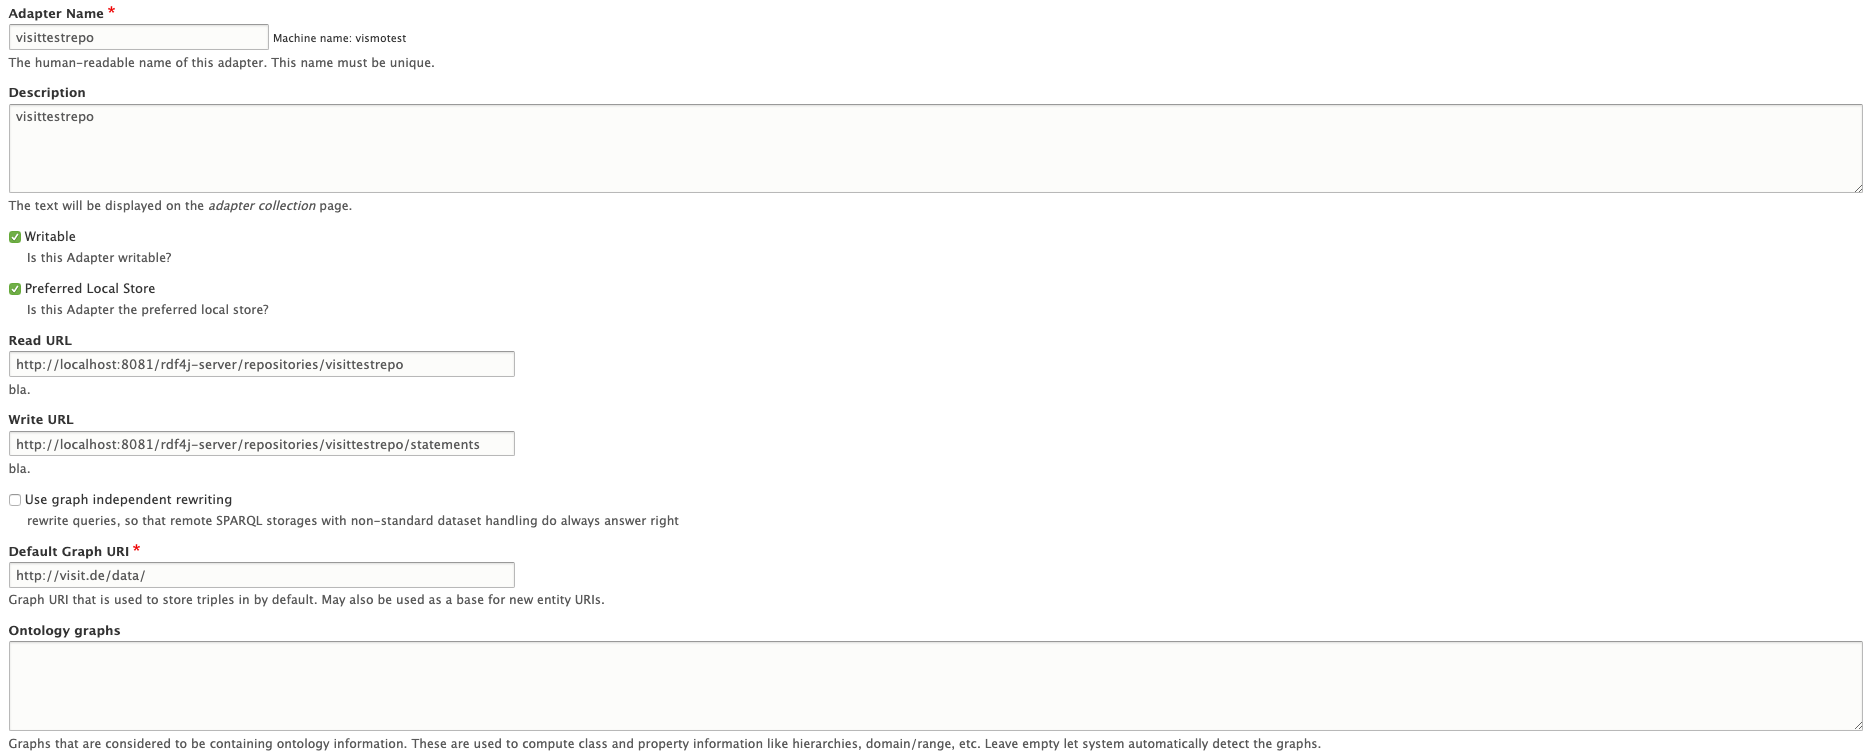
\includegraphics[width=1.0\textwidth,height=0.4\textwidth]{Figures/berndl/adapter1}
    \caption{\label{fig:adapter1} Übersicht der Konfiguration eines \wisski Salz Adapters, Teil 1.}
\end{sidewaysfigure}

\begin{sidewaysfigure}
    %\centering
    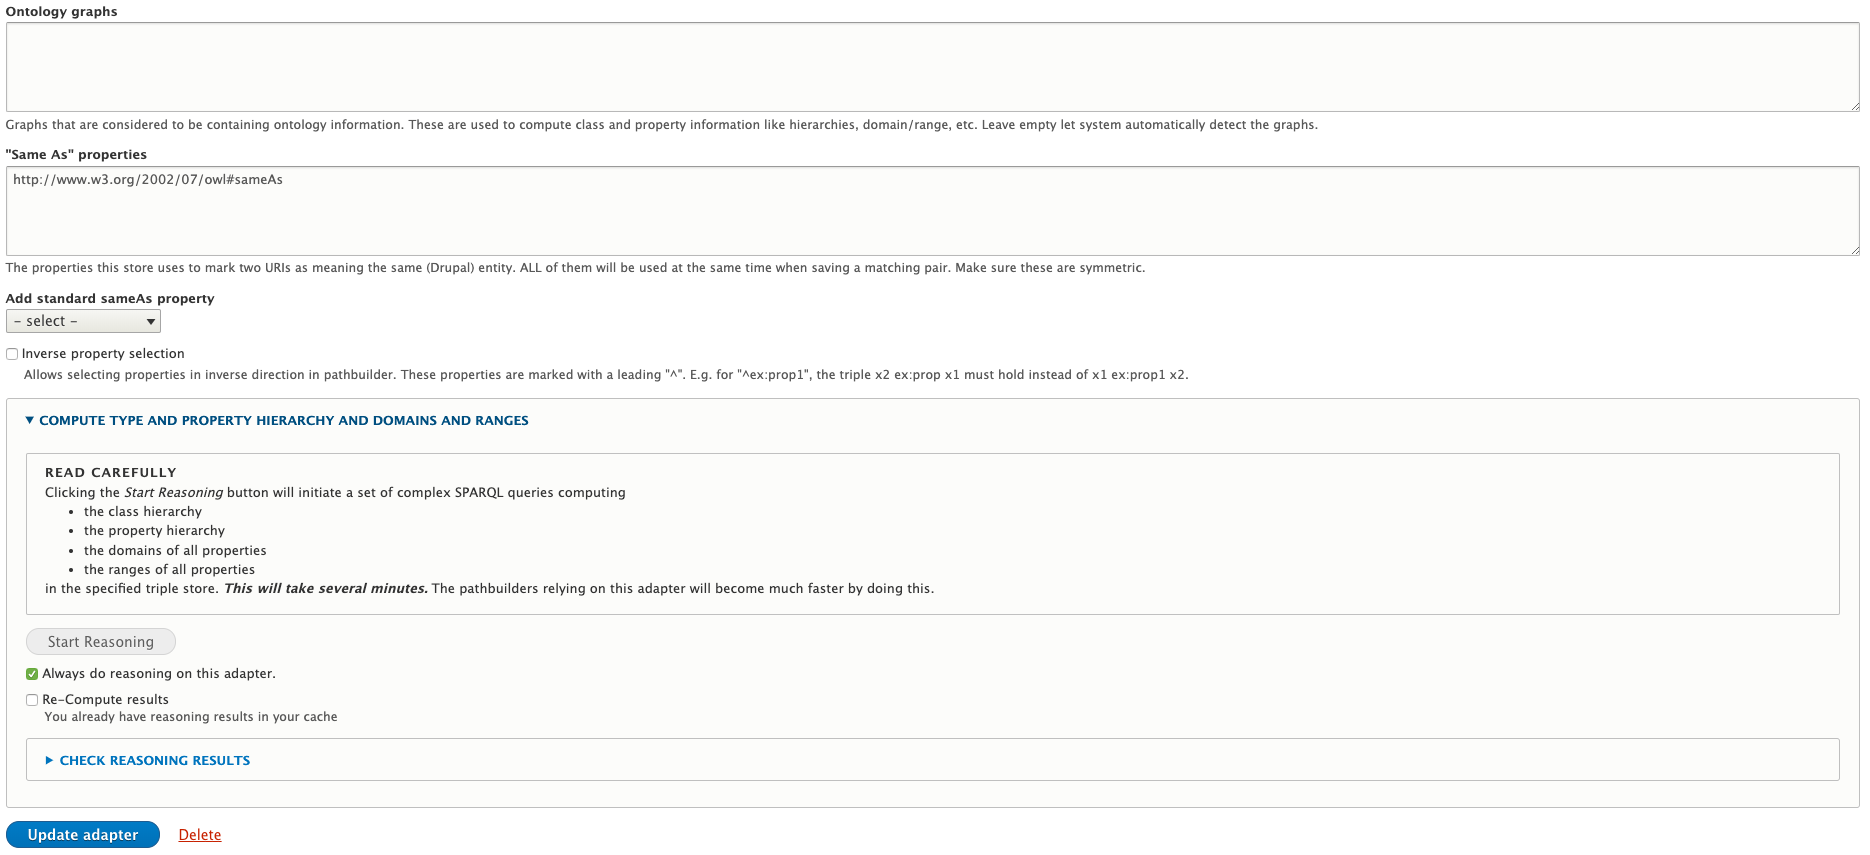
\includegraphics[width=1.0\textwidth,height=0.4\textwidth]{Figures/berndl/adapter3}
    \caption{\label{fig:adapter2} Übersicht der Konfiguration eines \wisski Salz Adapters, Teil 2.}
\end{sidewaysfigure}

\begin{sidewaysfigure}
    %\centering
    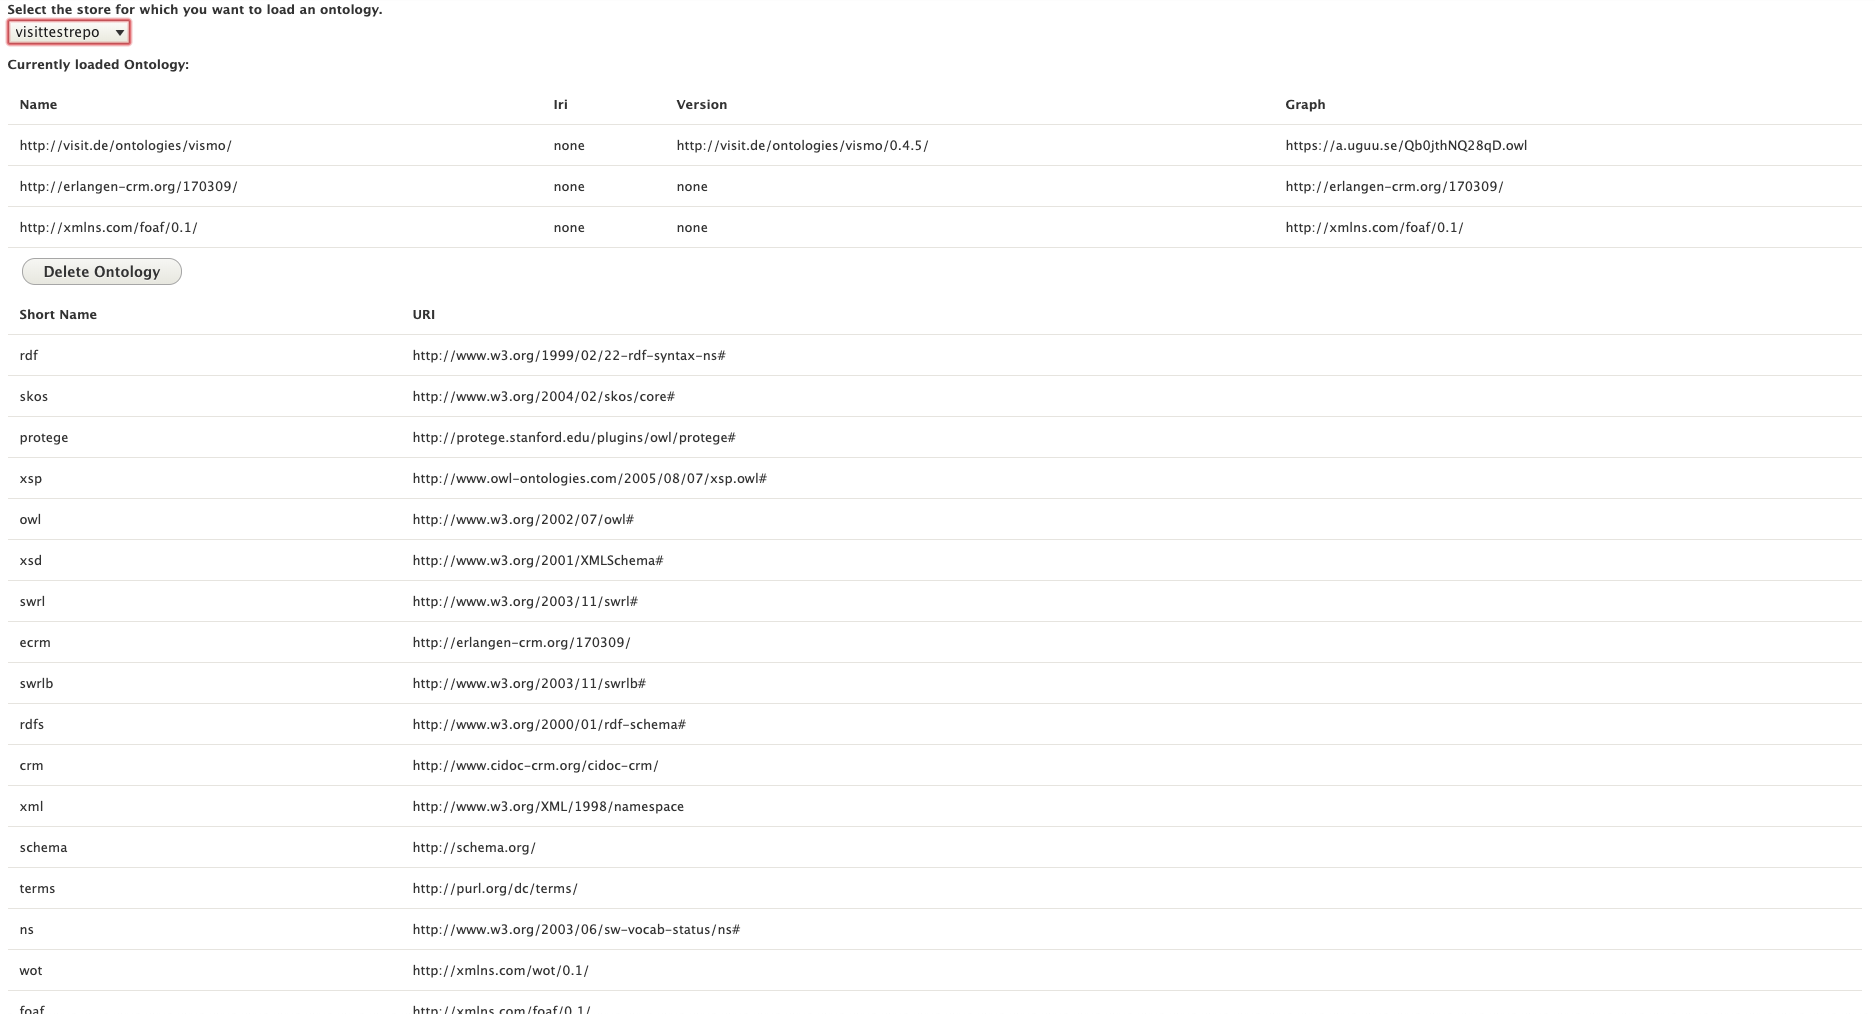
\includegraphics[width=1.0\textwidth,height=0.4\textwidth]{Figures/berndl/wisskiontology}
    \caption{\label{fig:wisskiontology} Detailansicht einer definierten Ontology im \wisski System am Beispiel VisMo für das ViSIT Projekt.}
\end{sidewaysfigure}

\begin{sidewaysfigure}
    %\centering
    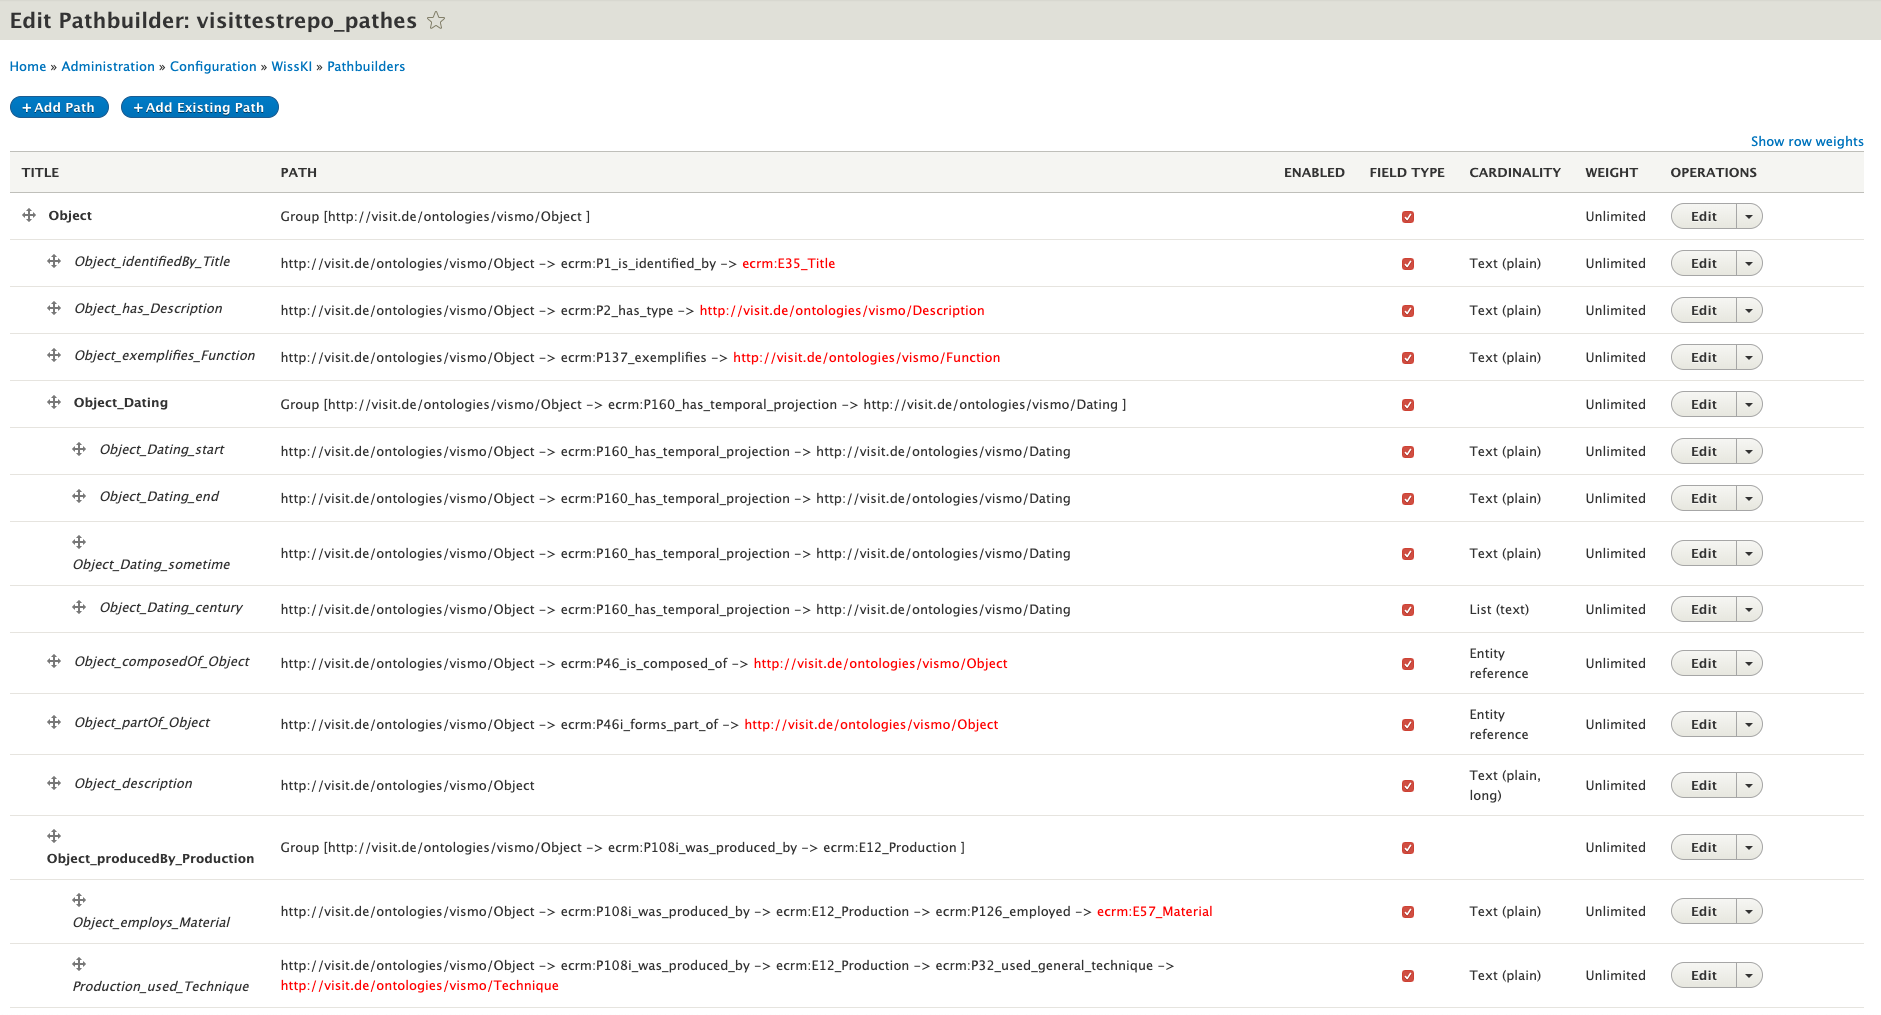
\includegraphics[width=1.0\textwidth,height=0.4\textwidth]{Figures/berndl/pathbuilder}
    \caption{\label{fig:pathbuilder} Übersicht der ersten Pfade des für das \visit Projekt definierten Pathbuilders.}
\end{sidewaysfigure}

\begin{figure}[htb]
    \centering
    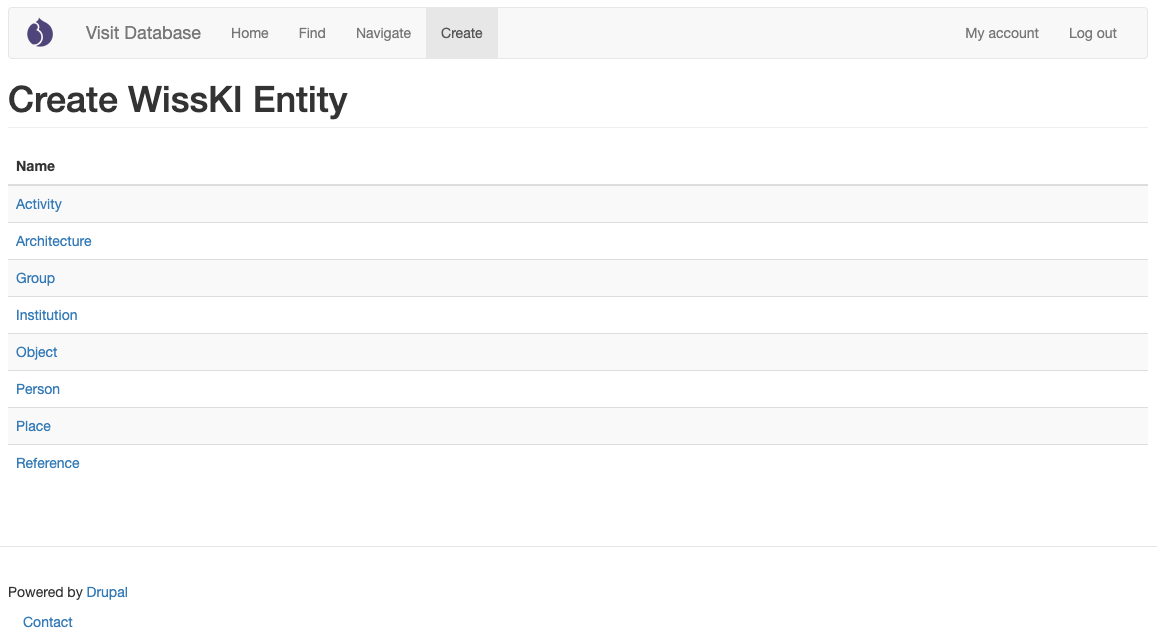
\includegraphics[width=\textwidth]{Figures/berndl/wisskiCreate}
    \caption{\label{fig:wisskiCreate} Ausgangs-Interface zum Erzeugen einer Hauptentität im \wisski System.}
\end{figure}

\begin{sidewaysfigure}
    %\centering
    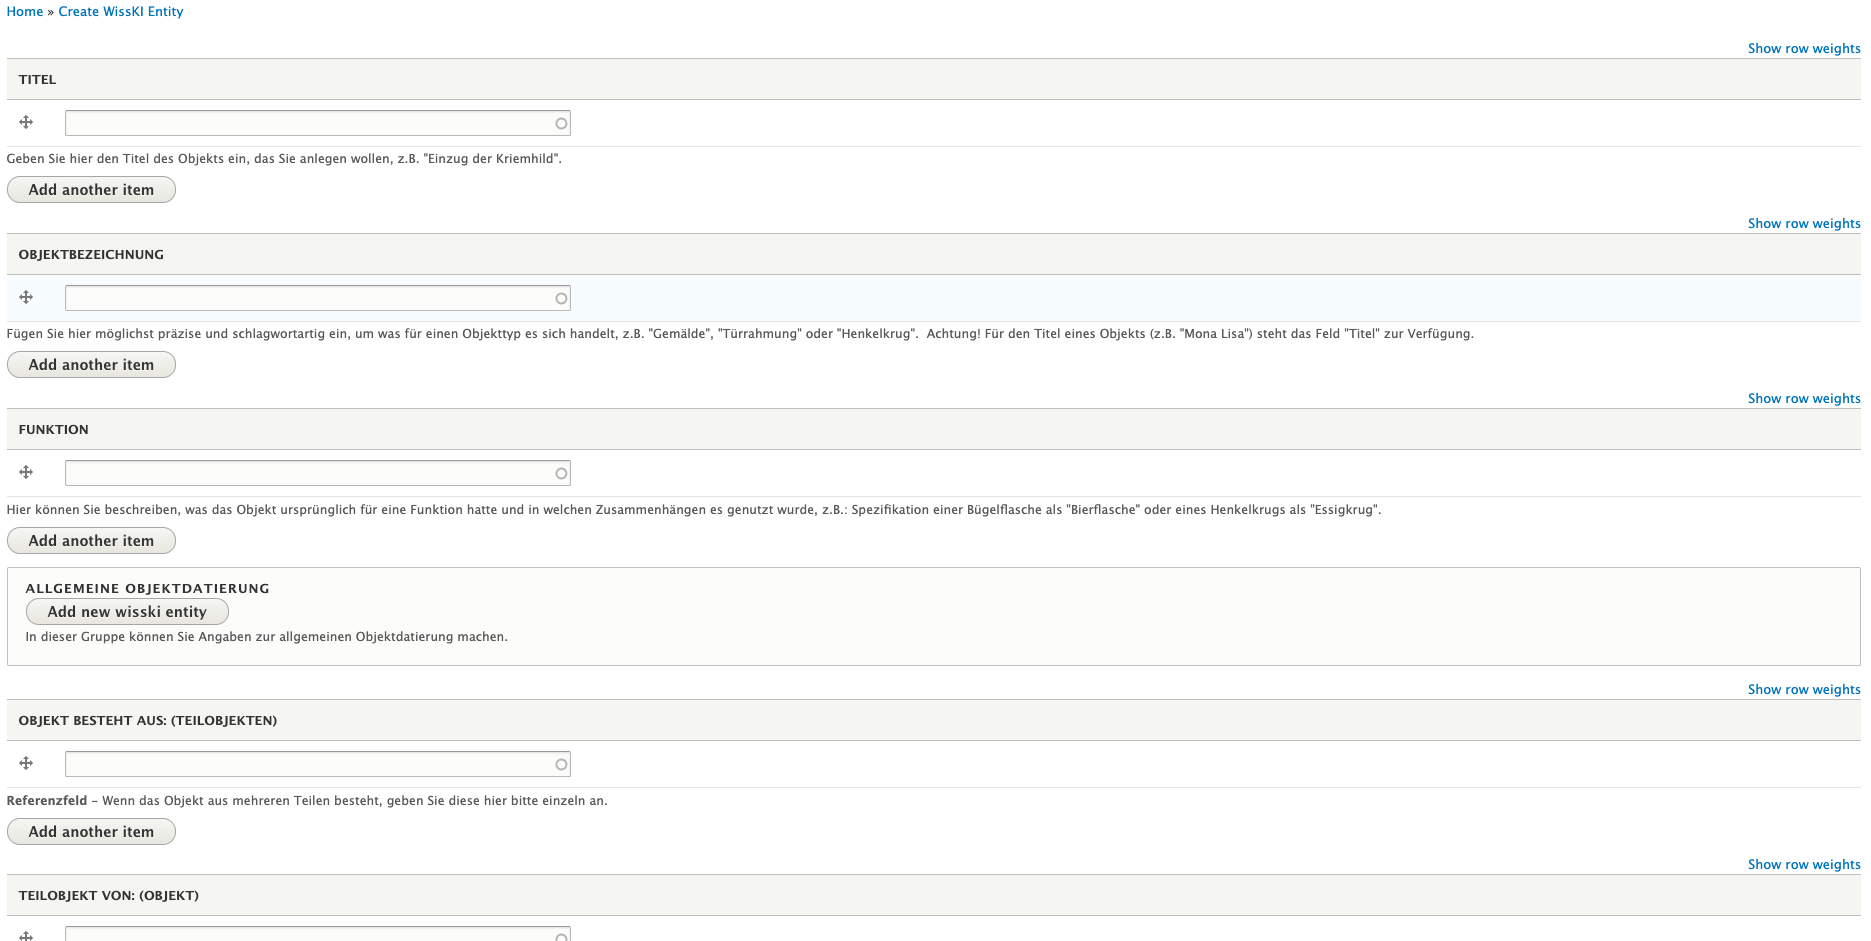
\includegraphics[width=1.0\textwidth,height=0.4\textwidth]{Figures/berndl/wisskiCreateObject}
    \caption{\label{fig:wisskiCreateObject} Eingabe-Interface für ein Ausstellungsobjekt im \visit \wisski System.}
\end{sidewaysfigure}

\begin{figure}[htb]
    \centering
    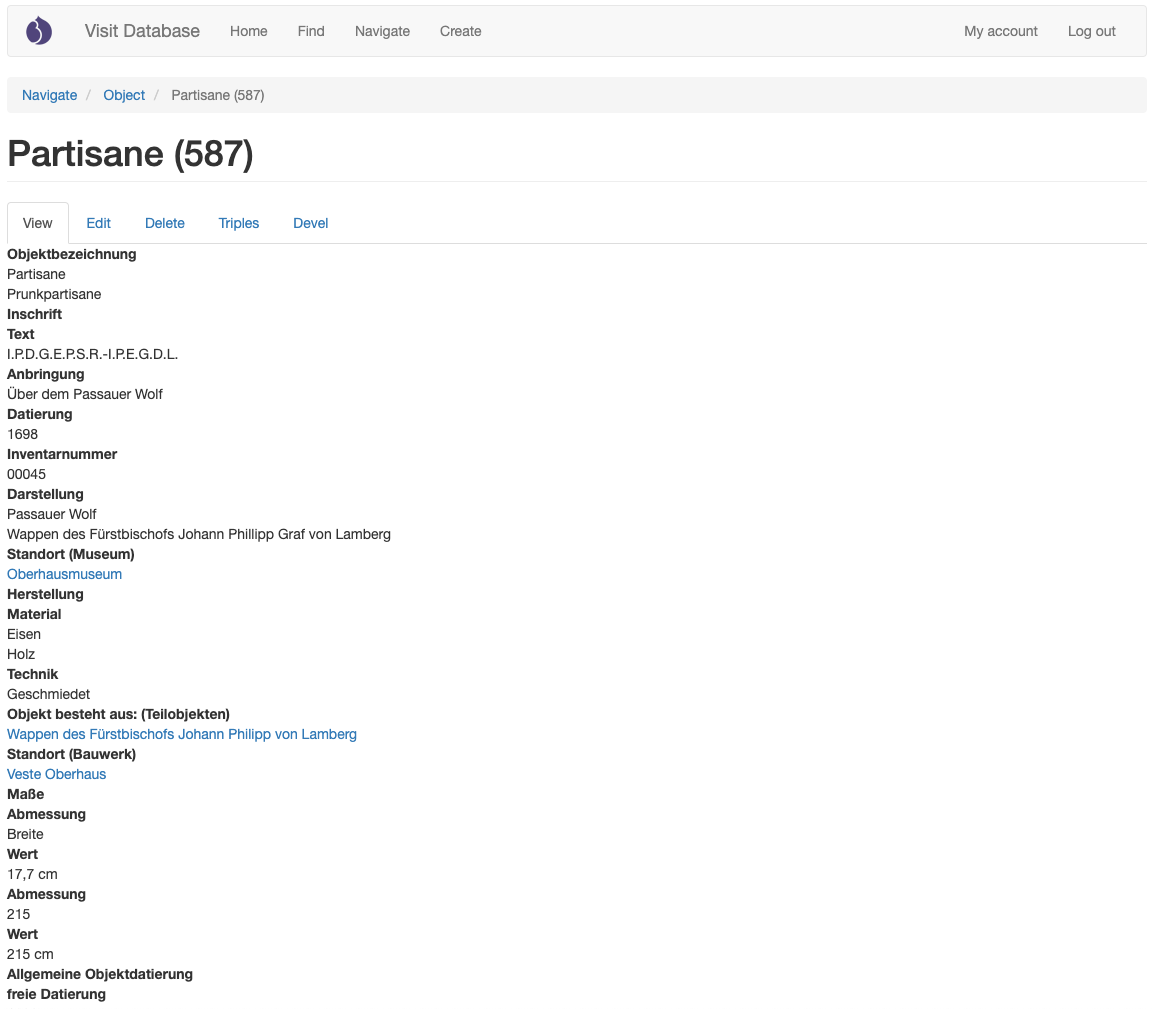
\includegraphics[width=\textwidth]{Figures/berndl/wisskiViewObject}
    \caption{\label{fig:wisskiViewObject} Beispiel Ausgabe-Interface einer Partisane des \visit \wisski Systems.}
\end{figure}

\begin{lstlisting}[caption={JSON \q{Schema} der ViSIT Daten, die über die REST API ausgespielt werden.},label={lst:json},captionpos=b,language=xml]
	{
  "Object": {
    "type": "http://visit.de/ontologies/vismo/Object",
    "object_identifiedby_title": "string",
    "object_has_description": "string",
    "object_exemplifies_function": "string",
    "object_inventory_number": "string",
    "object_description": "string_long",
    "object_comment": "string_long",
    "object_keyword": "string",
    "object_iconography": "string",
    "object_literature": "string_long",
    "object_current_owner": "entity_reference (http://visit.de/ontologies/vismo/Institution)",
    "object_current_location": "entity_reference (http://visit.de/ontologies/vismo/Institution)",
    "object_currentlocation_arch": "entity_reference (http://visit.de/ontologies/vismo/Architecture)",
    "object_composedof_object": "entity_reference (http://visit.de/ontologies/vismo/Object)",
    "object_partof_object": "entity_reference (http://visit.de/ontologies/vismo/Object)",
    "object_tookpartin_activity": "entity_reference (http://visit.de/ontologies/vismo/Activity)",
    "object_depicts_person": "entity_reference (http://visit.de/ontologies/vismo/Person)",
    "object_depicts_architecture": "entity_reference (http://visit.de/ontologies/vismo/Architecture)",
    "object_depicts_place": "entity_reference (http://visit.de/ontologies/vismo/Place)",
    "object_depicts_activity": "entity_reference (http://visit.de/ontologies/vismo/Activity)",
    "object_helpfullinks": "string",
    "object_thumbnail": "image",
    "object_prefidentifier_inscriptio": {
      "type": "http://erlangen-crm.org/170309/E34_Inscription",
      "inscription_text": "string",
      "inscription_has_type": "string",
      "inscription_signature": "string",
      "inscription_mounting": "string",
      "inscription_date": "string"
    },
    "object_producedby_production": {
      "type": "http://erlangen-crm.org/170309/E12_Production",
      "object_employs_material": "string",
      "production_used_technique": "string",
      "production_doneby_person": "entity_reference (http://visit.de/ontologies/vismo/Person)",
      "production_doneby_group": "entity_reference (http://visit.de/ontologies/vismo/Group)",
      "production_tookplaceat_place": "entity_reference (http://visit.de/ontologies/vismo/Place)",
      "production_dating": {
        "object_prod_dating_start": "string",
        "object_prod_dating_end": "string",
        "production_date_sometime": "string",
        "object_prod_dating_century": "list_string"
      }
    },
    "object_has_dimension": {
      "type": "http://erlangen-crm.org/170309/E54_Dimension",
      "dimension_has_measurementunit": "string",
      "dimension_hasvalue": "string"
    },
    "object_transferred_custody": {
      "type": "http://erlangen-crm.org/170309/E10_Transfer_of_Custody",
      "custody_receiving_person": "entity_reference (http://visit.de/ontologies/vismo/Person)",
      "custody_receiving_group": "entity_reference (http://visit.de/ontologies/vismo/Group)",
      "custody_from_person": "entity_reference (http://visit.de/ontologies/vismo/Person)",
      "custody_from_group": "entity_reference (http://visit.de/ontologies/vismo/Group)",
      "object_toc_dating": {
        "object_toc_dating_exact": "datetime",
        "object_toc_dating_start": "string",
        "object_toc_dating_end": "string",
        "object_toc_dating_sometime": "string",
        "object_toc_dating_century": "list_string"
      }
    },
    "object_dating": {
      "type": "http://visit.de/ontologies/vismo/Dating",
      "object_dating_start": "string",
      "object_dating_end": "string",
      "object_dating_sometime": "string",
      "object_dating_century": "list_string"
    },
    "object_refentry": {
      "type": "http://visit.de/ontologies/vismo/ReferenceEntry",
      "object_refentry_pages": "string",
      "object_refentry_in_reference": "entity_reference (http://visit.de/ontologies/vismo/Reference)"
    },
    "object_digitalrepresentation": {
      "type": "http://visit.de/ontologies/vismo/DigitalRepresentation",
      "object_dr_technicalmetadata": "string_long"
    }
  },
  "Person": {
    "type": "http://visit.de/ontologies/vismo/Person",
    "person_idby_actorappel": "string",
    "person_hastype_profession": "string",
    "person_firstname": "string",
    "person_lastname": "string",
    "person_pseudonym": "string",
    "person_alternatename": "string",
    "person_carries_title": "string",
    "person_comment": "string_long",
    "person_description": "string_long",
    "person_keyword": "string",
    "person_iconography": "string",
    "person_parentof_person": "entity_reference (http://visit.de/ontologies/vismo/Person)",
    "person_ischildof_person": "entity_reference (http://visit.de/ontologies/vismo/Person)",
    "person_ownerof_architecture": "entity_reference (http://visit.de/ontologies/vismo/Architecture)",
    "person_motiv_arch_production": "entity_reference (http://visit.de/ontologies/vismo/Architecture)",
    "person_carriedout_arch_prod": "entity_reference (http://visit.de/ontologies/vismo/Architecture)",
    "person_infld_arch_production": "entity_reference (http://visit.de/ontologies/vismo/Architecture)",
    "person_motiv_structevol": "entity_reference (http://visit.de/ontologies/vismo/Architecture)",
    "person_carriedout_structevol": "entity_reference (http://visit.de/ontologies/vismo/Architecture)",
    "person_infl_structevol": "entity_reference (http://visit.de/ontologies/vismo/Architecture)",
    "person_depictedon_object": "entity_reference (http://visit.de/ontologies/vismo/Object)",
    "person_participatedin_activity": "entity_reference (http://visit.de/ontologies/vismo/Activity)",
    "person_receivedcustody_object": "entity_reference (http://visit.de/ontologies/vismo/Object)",
    "person_lostcustodyof_object": "entity_reference (http://visit.de/ontologies/vismo/Object)",
    "person_helpfullinks": "string",
    "person_thumbnail": "image",
    "person_birth": {
      "type": "http://erlangen-crm.org/170309/E67_Birth",
      "person_mother": "entity_reference (http://visit.de/ontologies/vismo/Person)",
      "person_father": "entity_reference (http://visit.de/ontologies/vismo/Person)",
      "person_birthplace": "entity_reference (http://visit.de/ontologies/vismo/Place)",
      "person_birth_dating": {
        "person_birth_dating_exact": "datetime",
        "person_birth_dating_start": "string",
        "person_birth_dating_end": "string",
        "person_birth_dating_sometime": "string"
      }
    },
    "person_death": {
      "type": "http://erlangen-crm.org/170309/E69_Death",
      "person_deathplace": "entity_reference (http://visit.de/ontologies/vismo/Place)",
      "person_death_dating": {
        "person_death_dating_exact": "datetime",
        "person_death_dating_start": "string",
        "person_death_dating_end": "string",
        "person_death_dating_sometime": "string"
      }
    },
    "person_marriage": {
      "type": "http://visit.de/ontologies/vismo/Marriage",
      "marriage_partner_person": "entity_reference (http://visit.de/ontologies/vismo/Person)",
      "marriage_begin_dating": {
        "marriage_begin_dating_exact": "datetime",
        "marriage_begin_dating_start": "string",
        "marriage_begin_dating_end": "string",
        "marriage_begin_dating_sometime": "string"
      },
      "marriage_end_dating": {
        "marriage_end_dating_exact": "datetime",
        "marriage_end_dating_start": "string",
        "marriage_end_dating_end": "string",
        "marriage_end_dating_sometime": "string"
      }
    },
    "person_refentry": {
      "type": "http://visit.de/ontologies/vismo/ReferenceEntry",
      "person_refentry_pages": "string",
      "person_refentry_in_reference": "entity_reference (http://visit.de/ontologies/vismo/Reference)"
    },
    "person_digitalrepresentation": {
      "type": "http://visit.de/ontologies/vismo/DigitalRepresentation",
      "person_dr_technicalmetadata": "string_long"
    }
  },
  "Architecture": {
    "type": "http://visit.de/ontologies/vismo/Architecture",
    "architecture_idby_title": "string",
    "arch_sacraltype": "string",
    "arch_has_seculartype": "string",
    "arch_bishopricaffiliation": "string",
    "arch_geographicaffiliation": "string",
    "arch_orderaffiliation": "string",
    "architecture_description": "string_long",
    "architecture_comment": "string_long",
    "architecture_keyword": "string",
    "architecture_iconography": "string",
    "architecture_innerdescription": "string_long",
    "architecture_outerdescription": "string_long",
    "architecture_depictedby_object": "entity_reference (http://visit.de/ontologies/vismo/Object)",
    "architecture_buildinghistory": "string_long",
    "arch_currentlyholds_object": "entity_reference (http://visit.de/ontologies/vismo/Object)",
    "architecture_exemplify_function": "string",
    "architecture_location_place": "entity_reference (http://visit.de/ontologies/vismo/Place)",
    "arch_currentowner_person": "entity_reference (http://visit.de/ontologies/vismo/Person)",
    "arch_currentowner_group": "entity_reference (http://visit.de/ontologies/vismo/Group)",
    "arch_currentowner_institution": "entity_reference (http://visit.de/ontologies/vismo/Institution)",
    "architecture_contains_arch": "entity_reference (http://visit.de/ontologies/vismo/Architecture)",
    "architecture_fallswithin_arch": "entity_reference (http://visit.de/ontologies/vismo/Architecture)",
    "architecture_tookpartin_activity": "entity_reference (http://visit.de/ontologies/vismo/Activity)",
    "architecture_helpfullinks": "string",
    "architecture_thumbnail": "image",
    "arch_producedby_production": {
      "type": "http://erlangen-crm.org/170309/E12_Production",
      "production_motivatedby_person": "entity_reference (http://visit.de/ontologies/vismo/Person)",
      "production_carriedoutby_person": "entity_reference (http://visit.de/ontologies/vismo/Person)",
      "production_inflby_person": "entity_reference (http://visit.de/ontologies/vismo/Person)",
      "arch_prod_motivatedby_group": "entity_reference (http://visit.de/ontologies/vismo/Group)",
      "arch_prod_carriedoutby_group": "entity_reference (http://visit.de/ontologies/vismo/Group)",
      "arch_prod_inflby_group": "entity_reference (http://visit.de/ontologies/vismo/Group)",
      "arch_production_dating": {
        "arch_prod_dating_start": "string",
        "arch_prod_dating_end": "string",
        "archproduction_sometime": "string",
        "arch_prod_dating_century": "list_string"
      }
    },
    "arch_modifiedby_structevolution": {
      "type": "http://visit.de/ontologies/vismo/StructuralEvolution",
      "structuralevolution_idby_title": "string",
      "structuralevolution_description": "string_long",
      "structuralevolution_comment": "string_long",
      "structevol_exemplifies_function": "string",
      "structevol_motivatedby_person": "entity_reference (http://visit.de/ontologies/vismo/Person)",
      "structevol_carriedoutby_person": "entity_reference (http://visit.de/ontologies/vismo/Person)",
      "structevol_influencedby_person": "entity_reference (http://visit.de/ontologies/vismo/Person)",
      "structevol_motivby_group": "entity_reference (http://visit.de/ontologies/vismo/Group)",
      "structevol_carriedoutby_group": "entity_reference (http://visit.de/ontologies/vismo/Group)",
      "structevol_inflby_group": "entity_reference (http://visit.de/ontologies/vismo/Group)",
      "arch_structevol_dating": {
        "arch_structevol_dating_start": "string",
        "arch_structevol_dating_end": "string",
        "arch_evol_dat_sometime": "string",
        "arch_structevol_dating_century": "list_string"
      }
    },
    "arch_refentry": {
      "type": "http://visit.de/ontologies/vismo/ReferenceEntry",
      "arch_refentry_pages": "string",
      "arch_refentry_in_reference": "entity_reference (http://visit.de/ontologies/vismo/Reference)"
    },
    "architecture_digitalrepresentati": {
      "type": "http://visit.de/ontologies/vismo/DigitalRepresentation",
      "architecture_dr_techmetadata": "string_long"
    }
  },
  "Place": {
    "type": "http://visit.de/ontologies/vismo/Place",
    "place_idby_placeappel": "string",
    "place_description": "string_long",
    "place_comment": "string_long",
    "place_keyword": "string",
    "place_iconography": "string",
    "place_holds_architecture": "entity_reference (http://visit.de/ontologies/vismo/Architecture)",
    "place_witnessed_activity": "entity_reference (http://visit.de/ontologies/vismo/Activity)",
    "place_wasbirthplaceof_person": "entity_reference (http://visit.de/ontologies/vismo/Person)",
    "place_wasdeathplaceof_person": "entity_reference (http://visit.de/ontologies/vismo/Person)",
    "place_isdepictedby_object": "entity_reference (http://visit.de/ontologies/vismo/Object)",
    "place_helpfullinks": "string",
    "place_thumbnail": "image",
    "place_refentry": {
      "type": "http://visit.de/ontologies/vismo/ReferenceEntry",
      "place_refentry_pages": "string",
      "place_refentry_in_reference": "entity_reference (http://visit.de/ontologies/vismo/Reference)"
    },
    "place_digitalrepresentation": {
      "type": "http://visit.de/ontologies/vismo/DigitalRepresentation",
      "place_dr_techmetadata": "string"
    }
  },
  "Institution": {
    "type": "http://visit.de/ontologies/vismo/Institution",
    "institution_idby_appel": "string",
    "institution_ownerof_arch": "entity_reference (http://visit.de/ontologies/vismo/Architecture)",
    "institution_fallswithin_place": "entity_reference (http://visit.de/ontologies/vismo/Place)",
    "institution_address": "string",
    "institution_owns_catalog": "entity_reference (http://visit.de/ontologies/vismo/Reference)",
    "institution_loc_catalog": "entity_reference (http://visit.de/ontologies/vismo/Reference)",
    "institution_helpfullinks": "string"
  },
  "Group": {
    "type": "http://visit.de/ontologies/vismo/Group",
    "group_idby_actorappel": "string",
    "group_keyword": "string",
    "group_iconography": "string",
    "group_produced_object": "entity_reference (http://visit.de/ontologies/vismo/Object)",
    "group_ownerof_architecture": "entity_reference (http://visit.de/ontologies/vismo/Architecture)",
    "group_motiv_arch_production": "entity_reference (http://visit.de/ontologies/vismo/Architecture)",
    "group_carriedout_arch_production": "entity_reference (http://visit.de/ontologies/vismo/Architecture)",
    "group_infl_arch_production": "entity_reference (http://visit.de/ontologies/vismo/Architecture)",
    "group_motiv_structevol": "entity_reference (http://visit.de/ontologies/vismo/Architecture)",
    "group_carriedout_structevol": "entity_reference (http://visit.de/ontologies/vismo/Architecture)",
    "group_infl_structevol": "entity_reference (http://visit.de/ontologies/vismo/Architecture)",
    "group_receivedcustodyof_object": "entity_reference (http://visit.de/ontologies/vismo/Object)",
    "group_lostcustodyof_object": "entity_reference (http://visit.de/ontologies/vismo/Object)",
    "group_refentry": {
      "type": "http://visit.de/ontologies/vismo/ReferenceEntry",
      "group_refentry_pages": "string",
      "group_refentry_in_reference": "entity_reference (http://visit.de/ontologies/vismo/Reference)"
    }
  },
  "Reference": {
    "type": "http://visit.de/ontologies/vismo/Reference",
    "reference_keyword": "string",
    "reference_has_type": "string",
    "reference_publisher": "string",
    "reference_series": "string",
    "reference_volume": "integer",
    "reference_pages": "integer",
    "reference_catalog_owner": "entity_reference (http://visit.de/ontologies/vismo/Institution)",
    "reference_catalog_location": "entity_reference (http://visit.de/ontologies/vismo/Institution)",
    "reference_title": {
      "type": "http://visit.de/ontologies/vismo/Title",
      "reference_title_title": "string",
      "reference_title_superordinate": "string"
    },
    "reference_producedby_production": {
      "type": "http://erlangen-crm.org/170309/E12_Production",
      "production_authorname": "string",
      "production_year": "integer",
      "ref_production_placeofpub": "string"
    },
    "reference_entry": {
      "type": "http://visit.de/ontologies/vismo/ReferenceEntry",
      "reference_entry_pages": "string",
      "reference_entry_about_activity": "entity_reference (http://visit.de/ontologies/vismo/Activity)",
      "reference_entry_about_arch": "entity_reference (http://visit.de/ontologies/vismo/Architecture)",
      "reference_entry_about_object": "entity_reference (http://visit.de/ontologies/vismo/Object)",
      "reference_entry_about_place": "entity_reference (http://visit.de/ontologies/vismo/Place)",
      "reference_entry_about_group": "entity_reference (http://visit.de/ontologies/vismo/Group)",
      "reference_entry_about_person": "entity_reference (http://visit.de/ontologies/vismo/Person)"
    },
    "reference_catalog_dating": {
      "type": "http://visit.de/ontologies/vismo/Dating",
      "catalog_exhibition_start": "datetime",
      "catalog_exhibition_end": "datetime"
    }
  },
  "Activity": {
    "type": "http://visit.de/ontologies/vismo/Activity",
    "activity_idby_title": "string",
    "activity_description": "string_long",
    "activity_comment": "string_long",
    "activity_keyword": "string",
    "activity_iconography": "string",
    "activity_hadparticipant_person": "entity_reference (http://visit.de/ontologies/vismo/Person)",
    "activity_used_architecture": "entity_reference (http://visit.de/ontologies/vismo/Architecture)",
    "activity_used_object": "entity_reference (http://visit.de/ontologies/vismo/Object)",
    "activity_tookplaceat_place": "entity_reference (http://visit.de/ontologies/vismo/Place)",
    "activity_isdepictedby_object": "entity_reference (http://visit.de/ontologies/vismo/Object)",
    "activity_helpfullinks": "string",
    "activity_thumbnail": "image",
    "activity_dating": {
      "type": "http://visit.de/ontologies/vismo/Dating",
      "activity_dating_exact": "datetime",
      "activity_dating_end": "string",
      "activity_dating_start": "string",
      "activity_dating_sometime": "string"
    },
    "activity_refentry": {
      "type": "http://visit.de/ontologies/vismo/ReferenceEntry",
      "activity_refentry_pages": "string",
      "activity_refentry_in_reference": "entity_reference (http://visit.de/ontologies/vismo/Reference)"
    },
    "activity_digitalrepresentation": {
      "type": "http://visit.de/ontologies/vismo/DigitalRepresentation",
      "activity_dr_techmetadata": "string"
    }
  }
}
\end{lstlisting}